\documentclass[aspectratio=169,babel]{beamer}

\usetheme{boxes}

\usepackage[utf8]{inputenc}
\usepackage[T1]{fontenc}
\usepackage{bm}        % standard math notation (fonts)
\usepackage{amsfonts}
\usepackage{amssymb}
\usepackage{amsmath}  % standard math notation (vectors/sets/...)
\usepackage[ngerman]{babel}
\usepackage[babel,german=quotes]{csquotes}
%\usepackage{listings}
\usepackage{graphicx}
%\usepackage{ulem}
\usepackage{hyperref}
\usepackage{graphicx} % eps graphics support
\usepackage{epsfig}
\usepackage{subfigure}
\usepackage{times}           % scalable fonts
\usepackage{docmute}
\usepackage{algorithm}
\usepackage{algpseudocode}	% for nice algorithm writing


\newcommand{\qq}[1]{\glqq #1\grqq{}}


% Rename Require and Ensure labes to Input and Output
\renewcommand{\algorithmicrequire}{\textbf{Eingabe:}}
\renewcommand{\algorithmicensure}{\textbf{Ausgabe:}}

% mod without Space issue
\newcommand{\Mod}[1]{\ \text{mod}\ #1}


% Make Math serif
\usefonttheme{professionalfonts}
\DeclareMathOperator{\vol}{vol}
\DeclareMathOperator{\OPT}{OPT}

\makeatletter
    \@ifdefinable{\rucksack}{\def\rucksack/{\textsc{Rucksack}}}
\makeatother

% Adds titles for each section using section name as title
\AtBeginSection[]{
  \begin{frame}
  \vfill
  \centering
  \begin{beamercolorbox}[sep=8pt,center,shadow=true,rounded=true]{title}
    \usebeamerfont{title}\insertsectionhead\par%
  \end{beamercolorbox}
  \vfill
  \end{frame}
}

\setbeamertemplate{footline}[page number]
\setbeamertemplate{section in toc}{\inserttocsectionnumber.~\inserttocsection}
%\setbeamertemplate{frametitle}[default][center]

\beamertemplatenavigationsymbolsempty

\title{Präsentations-Titel}
\author{Markus Bullmann, Thimo Eder, \\ Stefan Gerasch, Julius Hackel, Re Jis}
\date{\today}

\begin{document}
    \maketitle
    \begin{frame}
        \frametitle{Gliederung}
        \tableofcontents
    \end{frame}
    
    % !TeX encoding = UTF-8
\section{Einführung}

\begin{frame}{Einführung}
	\begin{minipage}[t][0.25\textheight]{1\textwidth}
		\centering
		\qq{I can't find an efficient algorithm, \\ but neither can all these famous people.} \\ --- \textit{Garey und Johnson} ---
	\end{minipage}
	\pause
	\begin{minipage}[t][0.5\textheight]{1\textwidth}
	\begin{itemize}
		\item Annahme für alle folgenden Überlegungen: NP $\neq$ P
		\item Ein Problem ist NP-schwer, wenn es keinen Algorithmus gibt, der
			\begin{itemize}
				\item	deterministisch,
				\item exakt für alle Eingaben und 
				\item	effizient für alle Eingaben arbeitet.
			\end{itemize}
		\end{itemize}
	\end{minipage}
\end{frame}

\begin{frame}{Auswege aus der NP-Vollständigkeit}
\begin{itemize}
	\item In der Praxis sind NP-vollständige Problem jedoch trotzdem gut lösbar
	\item Auflockerung der obigen Bedingungen
	\item Effizient für \st{alle} gewisse Eingaben 
	\begin{itemize}
		\item[] $\Rightarrow$ Pseudopolynomielle Algorithmen
	\end{itemize}
	\item \st{Exakte} Approximierte Lösung
	\begin{itemize}
		\item[] $\Rightarrow$ Polynomielle Approximationsschemata
	\end{itemize}
\end{itemize}
\end{frame}

\begin{frame}{\textsc{Rucksack}-Problem}
    \textsc{Rucksack} ist ein NP-vollständiges Problem \\~\\
    \pause
    Grundidee: \qq{Qual der Wahl}
    
    \begin{itemize}
        \item Ein Dieb raubt einen Laden aus, jedoch hat er für die Beute nur einen Rucksack dabei
        \item Im Laden findet er $n$ Gegenstände
        \item Der $i$-te Gegenstand hat den Wert $p_i$ und das Gewicht $w_i$
        \item Sein Rucksack kann höchstens das Gewicht $B$ tragen
        \item $p_i, w_i$ und $B$ sind natürliche Zahlen
    \end{itemize}
    \alert{Welche Gegenstände sollten für den maximalen Profit gewählt werden?} 
\end{frame}
\begin{frame}{Beispiel}
    \begin{figure}[ht]
    	\centering
    	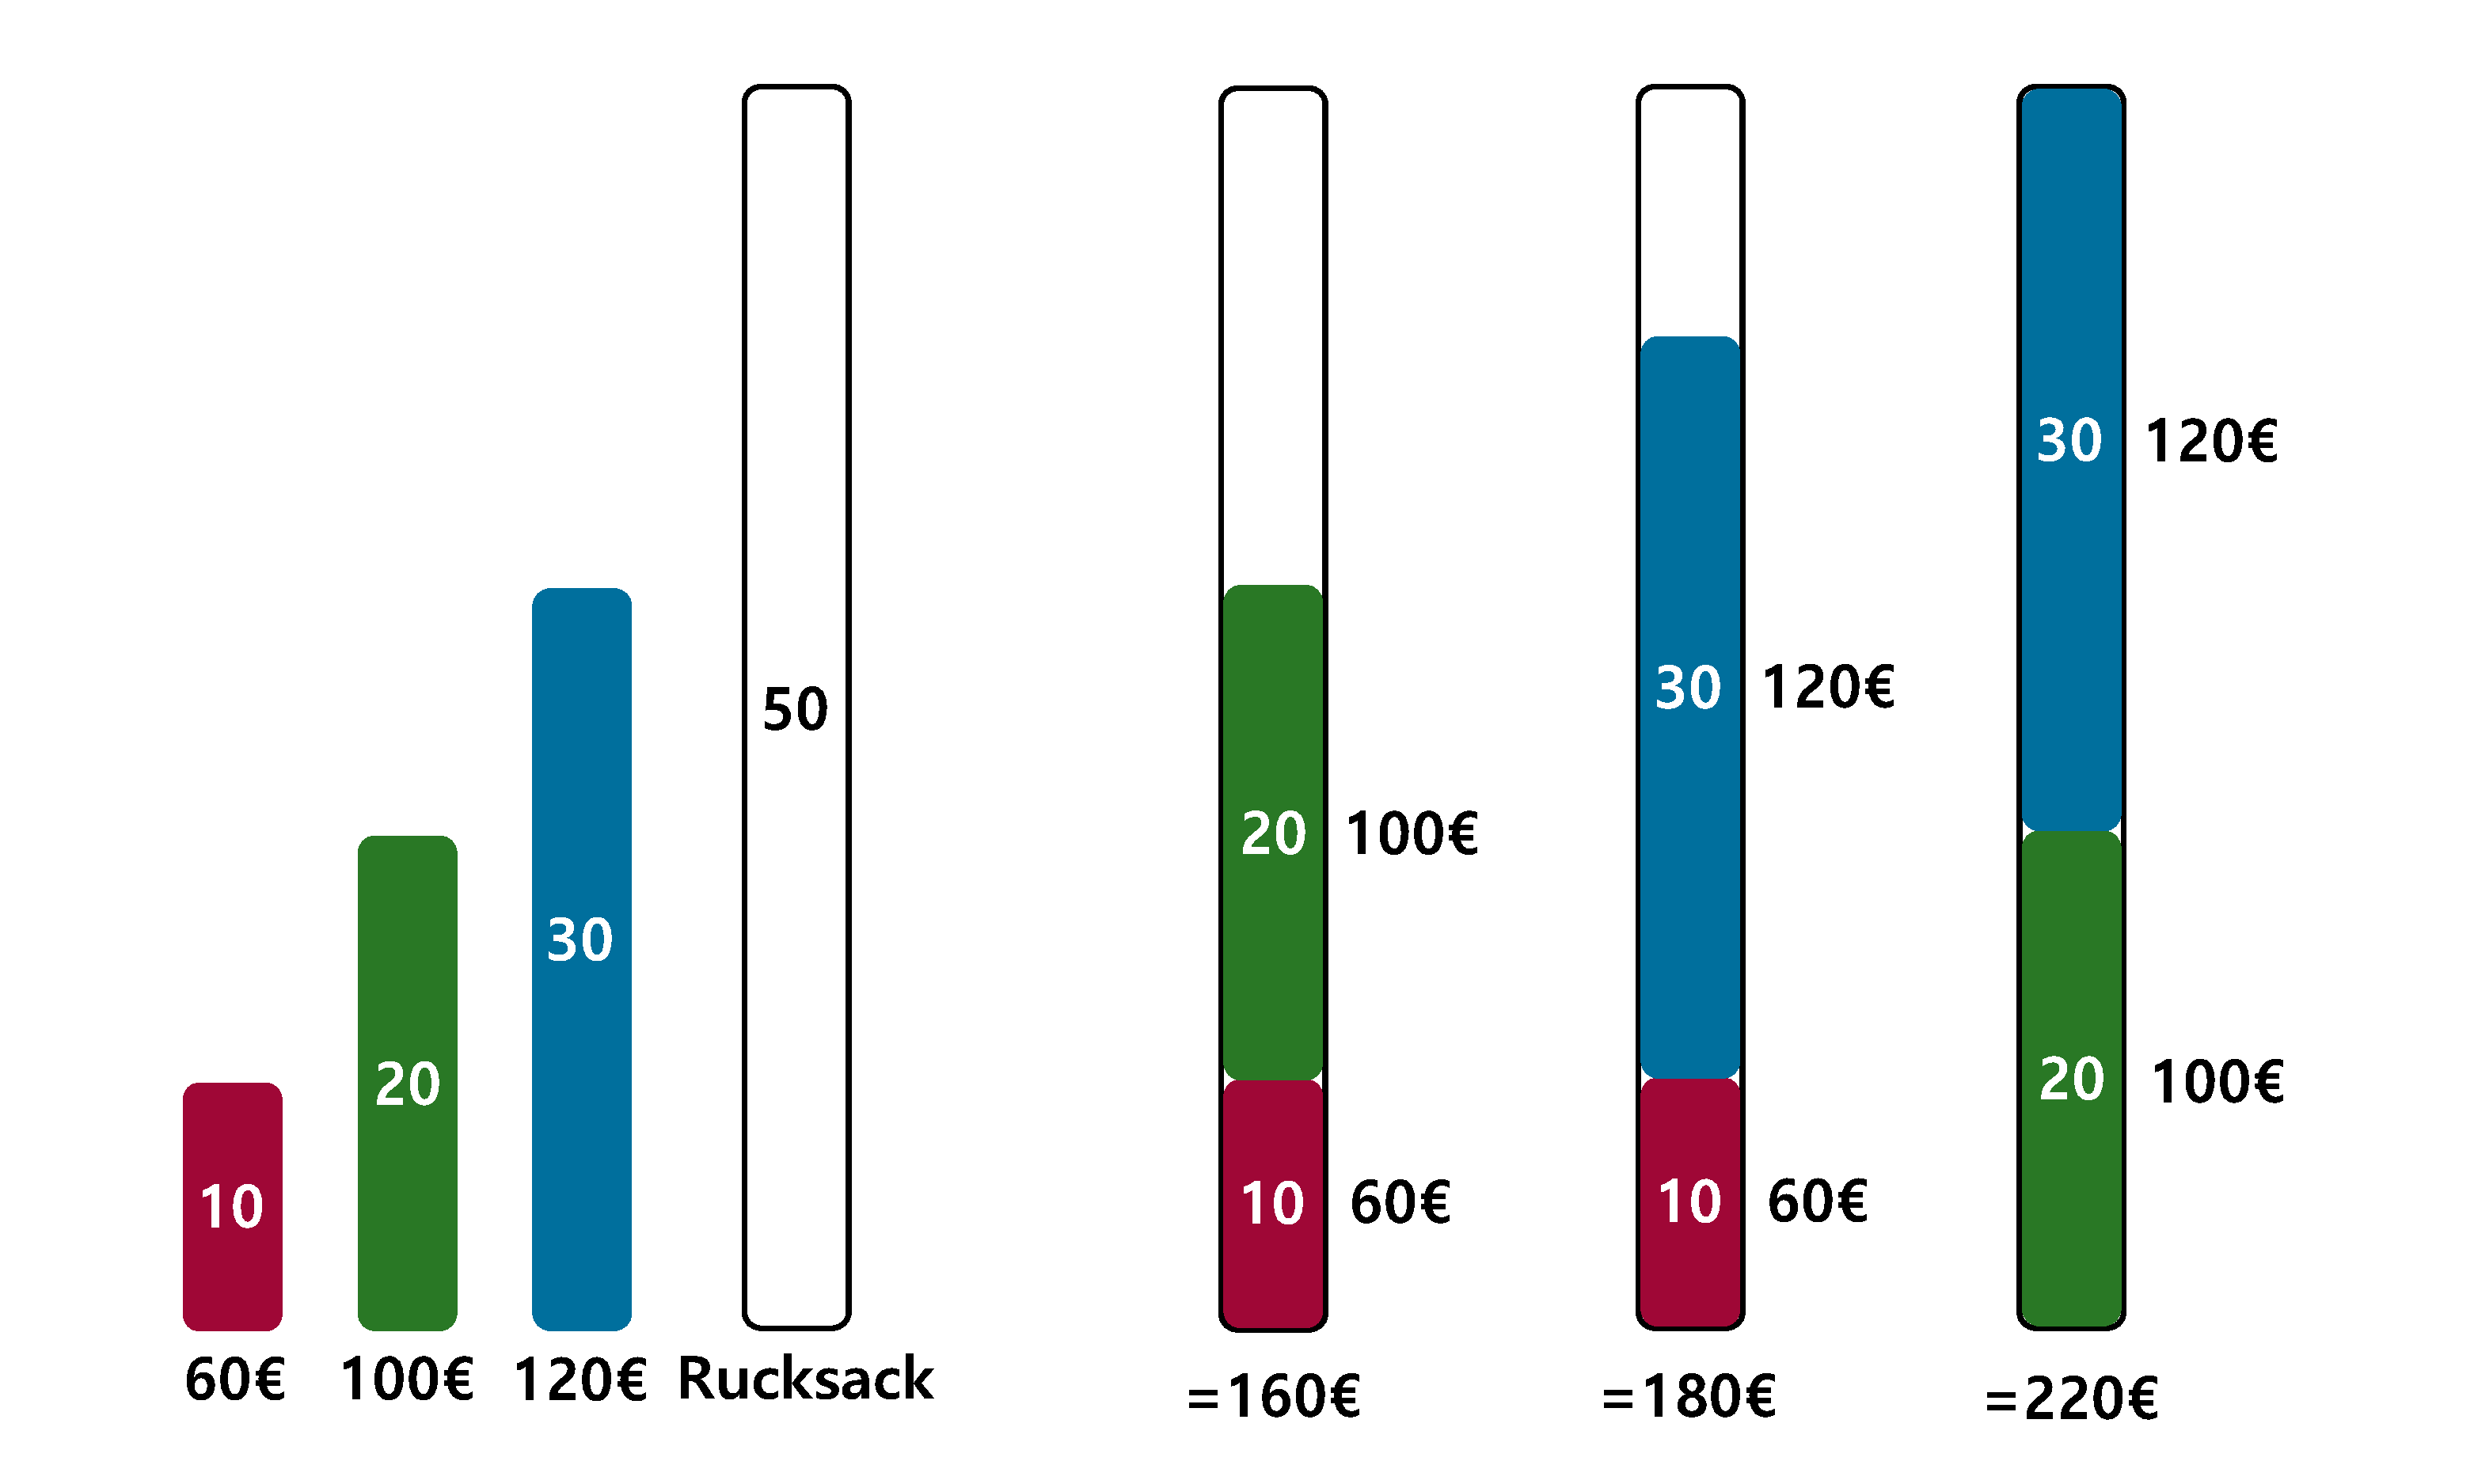
\includegraphics[width=0.9\textwidth]{img/Rucksack.pdf}
    	\caption{Rucksackproblem}
    	\label{fig:rucksack}
    \end{figure}
\end{frame}
\begin{frame}{\textsc{Rucksack}-Problem formal}
    \begin{itemize}
        \item $\begin{aligned}[t] \displaystyle
            \mathcal{D}=\{\langle W,w,p,B \rangle \mid & W=\{1,...,n\}, & \\
                                                                & w \colon W \to \mathbb{N}, & \\
                                                                & p \colon W \to \mathbb{N}, & \\
                                                                & B \in \mathbb{N}, & \\
                                                                & \forall i \in W \colon w_i \leq B\}
         \end{aligned}$
        
        \item $\displaystyle S( \langle W, w, p, B \rangle )=\{ A \subseteq W \mid \sum_{i\in A}{ w_i} \leq B \}$
        \item $\displaystyle f(A)=\sum_{i\in A}{p_i}$
        \item $\displaystyle \max$
    \end{itemize}
\end{frame}
\begin{frame}{0-1 \textsc{Rucksack}-Problem}
\begin{itemize}
	\item maximiere $\displaystyle \sum_{i=1}^{n}{x_i p_i}$
       
    \item unter der Bedingung $\displaystyle \sum_{i=1}^{n}{x_i w_i \leq B}$
       
     \item mit $x_i=1$ wenn Gegenstand $i$ im Rucksack enthalten ist, sonst $x_i=0$
\end{itemize}
\end{frame}
\begin{frame}{0-1 \textsc{Rucksack}-Problem}
\begin{itemize}
	\item Maximaler Profit ohne Überschreitung des Rucksackvolumen.
    \item Idee: Profit diskret erhöhen und prüfen ob mehr gehen würde.
    Hierzu benötigen wir eine Funktion die für einen bestimmten Wert $\alpha$ das minimal benötige Volumen zurück gibt.
    So können wir prüfen ob unser Rucksackvolumen $B$ bei einem bestimmten Profit $\alpha$ überschritten ist.
    
    \item Dynamische Lösung: Schritt für Schritt an die optimale Lösung heran arbeiten.
\end{itemize}
\end{frame}
\begin{frame}{0-1 \textsc{Rucksack}-Problem}
    Für $j \in \{0,1,...,n\}$ und $\alpha \in \mathbb{Z}$ sei $F_j(\alpha)$ das kleinste benötigte Rucksackvolumen, mit dem
    man einen Wert von mindestens $\alpha$ erzielen kann, wenn man die ersten $j$ Waren einpacken darf. 
    
    \begin{equation*}
        F_j(\alpha) = \min\{w(R) \mid R \subseteq \{1,...,j\}, p(R) \geq \alpha  \}
    \end{equation*}
    
    Rekursion:
    \begin{equation*}
        F_j(\alpha) = \begin{cases}
        0 & \text{für } \alpha\leq 0, j \in \{0,...,n \} \\
        \infty & \text{für } \alpha\geq 1, j = 0 \\
        \min\{F_{j-1}(\alpha-p_j) + w_j, F_{j-1}(\alpha) \} & \text{sonst}
        \end{cases}       
    \end{equation*}
\end{frame}

\begin{frame}{Algorithmus \textsc{DynRucksack}}
    Gesucht ist insgesamt also das größte $\alpha$, sodass $F_n(\alpha)$ noch in den Rucksack der Kapazität $B$
    passt, d.h. $\OPT(I)=\max\{ \alpha \mid F_n(\alpha) \leq B \}$.
    
\begin{algorithm}[H]
    \caption{Exakter \rucksack/ Algorithmus}
        \begin{algorithmic}
            \State $\alpha:=0;$
            \Repeat
            \State $\alpha:=\alpha+1;$
            \For{$j:=1$ \textbf{to} $n$}
            \State $F_j(\alpha):=\min\{F_{j-1}(\alpha-p_j)+w_j,F_{j-1}(\alpha)\};$
            \EndFor
            \Until{$B < F_n(\alpha)$}
            \State gib $\alpha-1$ aus$;$
        \end{algorithmic}
\end{algorithm}



\end{frame}
\begin{frame}{Komplexität von \textsc{DynRucksack}}
%    Innere Schleife: $n$-mal \\
%    Äußere Schleife: $\alpha$-mal \newline       
    $\mathcal{O}( n \cdot \alpha) = \mathcal{O}( n \cdot \OPT(I))$ \\~\\
    \pause    
    Es gilt $P_{\text{max}} \leq \text{OPT}(I) \leq n \cdot P_{\text{max}}$ 
    \quad mit $P_{\text{max}}=\max\{p_j \mid j \in \{1,...,n\}\}$ \\~\\
    \pause
    Warum?
    \begin{itemize}
        \item Untere Grenze: \\ Die minimale Rucksackfüllung beträgt $P_{\text{max}}$, da im schlimmsten Fall nur der wertvollste Gegenstand mitgenommen werden kann.
        \item Obere Grenze:  \\ Im Extremfall enthält die Rucksackfüllung alle $n$ Gegenstände, die alle den Preis $P_{\text{max}}$ haben. Somit ergibt sich der maximale Warenwert von $n \cdot P_{\text{max}}$.
    \end{itemize} ~\\
    
    $\Rightarrow \mathcal{O}( n \cdot n \cdot P_{\max}) = \mathcal{O}( n^2 \cdot P_{\max})$    
\end{frame}

    % !TeX encoding = UTF-8
\section{Pseudopolynomielle Algorithmen}

\begin{frame}{Pseudopolynomielle Algorithmen}
Definition:

Sei $\Pi$ ein kombinatorisches Optimierungsproblem, so dass für alle Instanzen $I$ gilt, dass alle in $I$ vorkommenden Zahlen natürliche Zahlen sind. Sei maxnr($I$) die größte in $I$ vorkommende Zahl. Ein Algorithmus für $\Pi$ heißt pseudopolynomiell, falls es ein Polynom poly(.,.)  gibt, so 
dass für alle Instanzen $I$ seine Laufzeit poly(|$I$| ,maxnr($I$)) ist. 

\end{frame}
\begin{frame}
Bedeutung:

\begin{itemize}
\item
Die Laufzeit ist polynomiell in der Eingabelänge und der größten vorkommenden Zahl beschränkt

\item
Das Problem ist (unter der Annahme P $\neq$ PN) nur für Eingaben mit großen Zahlen schwer lösbar, sonst effizient

\end{itemize}

Verwendung:
\begin{itemize}
\item
Macht NP-Vollständige Probleme unter gewissen Einschränkungen effizient lösbar

\end{itemize}
\end{frame}

\begin{frame}
\textbf{Verständliches Beispiel:}
\textbf{Primzahltest}

\begin{itemize}
\item
Testet, ob eine gegebene Zahl eine Primzahl ist
\item
Klassisches Verfahren: Teile die Eingabe $n$ durch alle Primzahlen mit $2 \leq p \leq \sqrt{n}$
\end{itemize}

\begin{algorithm}[H]
\caption{Naiver Primzahltest}
    \begin{algorithmic}
        \Require{ Zahl $n$}
        \Ensure{$true$ falls $n$ zusammengesetzt wurde, $false$ sonst.}
        \Function{IsPrim}{$n$}
            \For{Primzahlen $p$ mit $2 \leq p \leq \sqrt{n}$}
            \If{$n \mod{p} = 0$}
                  	\State return $true$
            \Else
                  	\State return $false$
            \EndIf
            \EndFor
        \EndFunction
    \end{algorithmic}
\end{algorithm}
\end{frame}

\begin{frame}
Problem:

\begin{itemize}
\item
Benötigt n-2 Divisionen, die laufzeit ist also linear in n
\item
Aber: Komplexität wird in der Eingabelänge |$n$| berechnet
\item
Daher: Exponentielle Laufzeit, problematisch bei großen Eingaben
TODO: Erklären warum man Eingabelänge betrachtet (Mehr Bits usw!)
\end{itemize}
\end{frame}

\begin{frame}
Anwendung auf \textsc{Rucksack}
\newline

Algorithmus: \newline

\begin{algorithmic}
\State $\alpha:=0;$
\Repeat
	\State $\alpha:=\alpha+1;$
	\For{$j:=1$ \textbf{to} $n$}
		\State $F_j(\alpha):=\min\{F_{j-1}(\alpha-p_j)+\text{vol}(j),F_{j-1}(\alpha)\};$
	\EndFor
\Until{$B < F_n(\alpha)$}
\State gib $\alpha-1$ aus$;$
\end{algorithmic}

\end{frame}
    % !TeX encoding = UTF-8
\section{Approximationsschemata}

\begin{frame}{Approximationsschemata}	
    Lorem ipsum dolor sit amet, consectetuer adipiscing elit. Maecenas porttitor congue massa. Fusce posuere, magna sed pulvinar ultricies, purus lectus malesuada libero, sit amet commodo magna eros quis urna.
    Nunc viverra imperdiet enim. Fusce est. Vivamus a tellus.
    Pellentesque habitant morbi tristique senectus et netus et malesuada fames ac turpis egestas. Proin pharetra nonummy pede. Mauris et orci.
    Aenean nec lorem. In porttitor. Donec laoreet nonummy augue.
    Suspendisse dui purus, scelerisque at, vulputate vitae, pretium mattis, nunc. Mauris eget neque at sem venenatis eleifend. Ut nonummy.      
\end{frame}
    % !TeX encoding = UTF-8
\section{Unmöglichkeitsergebnisse}

\begin{frame}{Unmöglichkeitsergebnisse}
	 Wann stoßen Apprimationsschemata an ihre Grenzen?   
\end{frame}

\begin{frame}{Unmöglichkeitsergebnisse}
	Definition nach Wanka (S. 73, Definition 4.9) \newline
	
	Ein NP-vollständiges Entscheidungsproblem $L$ heißt stark NP-vollständig,  wenn es ein Polynom $q$ gibt, so dass $L_q = \{x\vert x \in L \text{ und } \maxnr(x) \leq q(\vert x \vert)\}$ NP-vollständig  ist. Gibt es kein solches Polynom, heißt $L$ schwach  NP-vollständig.
\end{frame}

\begin{frame}{Unmöglichkeitsergebnisse}
	Bedeutung
	\begin{itemize}
		\item Ist ein Entscheidungsproblem $L$ NP-vollständig und $\maxnr(x)$ polynomiell in der Länge der Eingabe $\vert x \vert$ beschränkt, so ist es stark NP-vollständig.
		\item D.h. trotz der Einschränkung, dass $\maxnr(x)$ nicht exponentiell werden darf, ist das Problem NP-vollständig und nicht in polynomieller Zeit lösbar.
		\item Gibt es kein solches Polynom, so ist das Problem $L$ schwach NP-vollständig.
	\end{itemize}
\end{frame}

\begin{frame}{Unmöglichkeitsergebnisse}
	Anders ausgedrückt
	\begin{itemize}
		\item Gibt es für ein NP-vollständiges Entscheidungsproblem $L$ keinen pseudopolynomiellen exakten Algorithmus, so ist das Problem stark NP-vollständig
		\item Voraussetzung: P $\neq$ NP\newline
	\end{itemize}
	\pause

	Enge Beziehung zwischen starker NP-Vollständigkeit und FPAS
	\begin{itemize}
		\item Gibt es ein Polynom $q(x_1,x_2)$, so dass für alle Probleminstanzen $I$ gilt, dass $\OPT(I) \le q(\vert I \vert, \maxnr(I))$ ist, dann folgt aus der Existenz eines FPAS für das Problem, dass es dafür auch einen pseudopolynomiellen exakten Algorithmus gibt.
		\item Gibt es für eine Optimierungsvariante eines stark NP-vollständigen Problems ein FPAS, dann ist P $=$ NP.
	\end{itemize}
\end{frame}
\begin{frame}
	Schlussfolgerung
	\begin{itemize}
		\item Ist N $\neq$ NP, so kann es für viele Optimierungsprobleme (\textsc{Clique}, Graphenfärbungsprobleme, TSP) keine streng polynomiellen Approximationsschemata geben. 
	\end{itemize}
	
\end{frame}
    \input{sections/05_fazit.tex}

\end{document}